\vspace*{8.5cm}

\begin{minipage}{1.0\textwidth}

\begin{flushright}
	\section{\huge{\underline{Project Description}}}
\end{flushright}
\end{minipage}

%Multicols package is used to declate multiple %columns in the document class of latex
% \begin{multicols}{No. of COLUMNS} 
\begin{multicols}{2}

		\subsection{Introduction}

%This paragraph contains the overview of the project.
			\lettrine{T}{he} Remote Display utilises a simple static scrolling LED display and make is accessible from a nearby location using the \gls{ble} feature of an Android phone. Using such a feature the user can modify the display at will and with ease, this reduces the time to manually reprogram the controlling unit and does not require any computer. Having remote access makes the display very handy for a users who keeps the display at a non accessible location. 
			
			The Remote Display works around a 16x8 RED \gls{led} matrix which is controlled by the \gls{mcu}.
			
		\subsection{Hardware}
			\subsubsection{MCU}
				The remote display is built around a ATmega328P \gls{avr} microcontroller. This \gls{mcu} is based on advanced RISC \cite{AtMega328P} architecture, 8 bit \gls{mcu} and 23 programmable \gls{io} lines. For controlling the \textsc{remote display} shift registers are used, 2 for Column and 1 for row, due to shift registers few \gls{mcu} \gls{io} lines are used.
			\subsubsection{LED Matrix}
				 Single colour  RED 5mm \gls{led} used to build the matrix, total of 128 \gls{led} required for 16x8 matrix. An array of transistors configured as switch to provide required current for each row of \gls{led} matrix.  

			\subsubsection{Power supply}
				The project utilises a transformerless capacitive power supply design. Such a design is helpful in reducing the overall cost of project and also utilises fewer components thus saving space and cost.
				
				
			
			\subsubsection{Input}
				 The project is aimed to dynamically modify the display commands through an input source like computer or \gls{ble}. Such a feature helps in modifying the display at will rather than modifying the source code.

\end{multicols}

\begin{figure*}		
	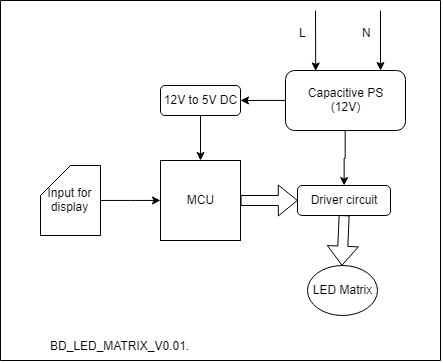
\includegraphics[scale = 0.3]{BD_LED_MATRIX_V1.png}
	\caption{Block Diagram V1.0}	
\end{figure*}	
	
\begin{multicols}{2}

\end{multicols}	 
			
				  



